\documentclass[11pt, a4paper]{article}
\usepackage[utf8]{inputenc}
\usepackage{minted}
\usepackage{graphicx}
\graphicspath{{./images/}}

\begin{document}
\title{Traffic Sign Classification}
\author{Samuel Navarro}
\date{\today}
\maketitle

\section{Data Set Summary and Exploration}%
\label{sec:data_set_summary_and_exploration}

\textbf{1. Provide a basic summary of the data set.}

The training set is 34799, the validation set is 4410 and the number of testing examples are 12630.

The total number of classes are 43 and the Images have a shape of 32, 32, 3. 

\textbf{2. Include an exploratory visualization of the dataset}

We can see that the data is unbalanced but given the obtainer accuracy, I don't think is necessary to augment the data. It could be done in the future to improve the accuracy further.

\begin{figure}[htb!]
	\centering
	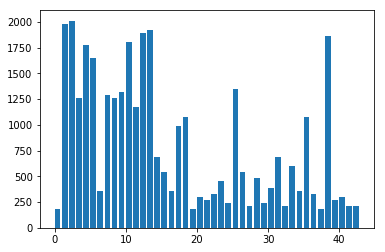
\includegraphics[width=0.8\linewidth]{count}
	\caption{count}
	\label{fig:count}
\end{figure}


Here's a visualization of the images with the given labels:


\begin{figure}[htb!]
	\centering
	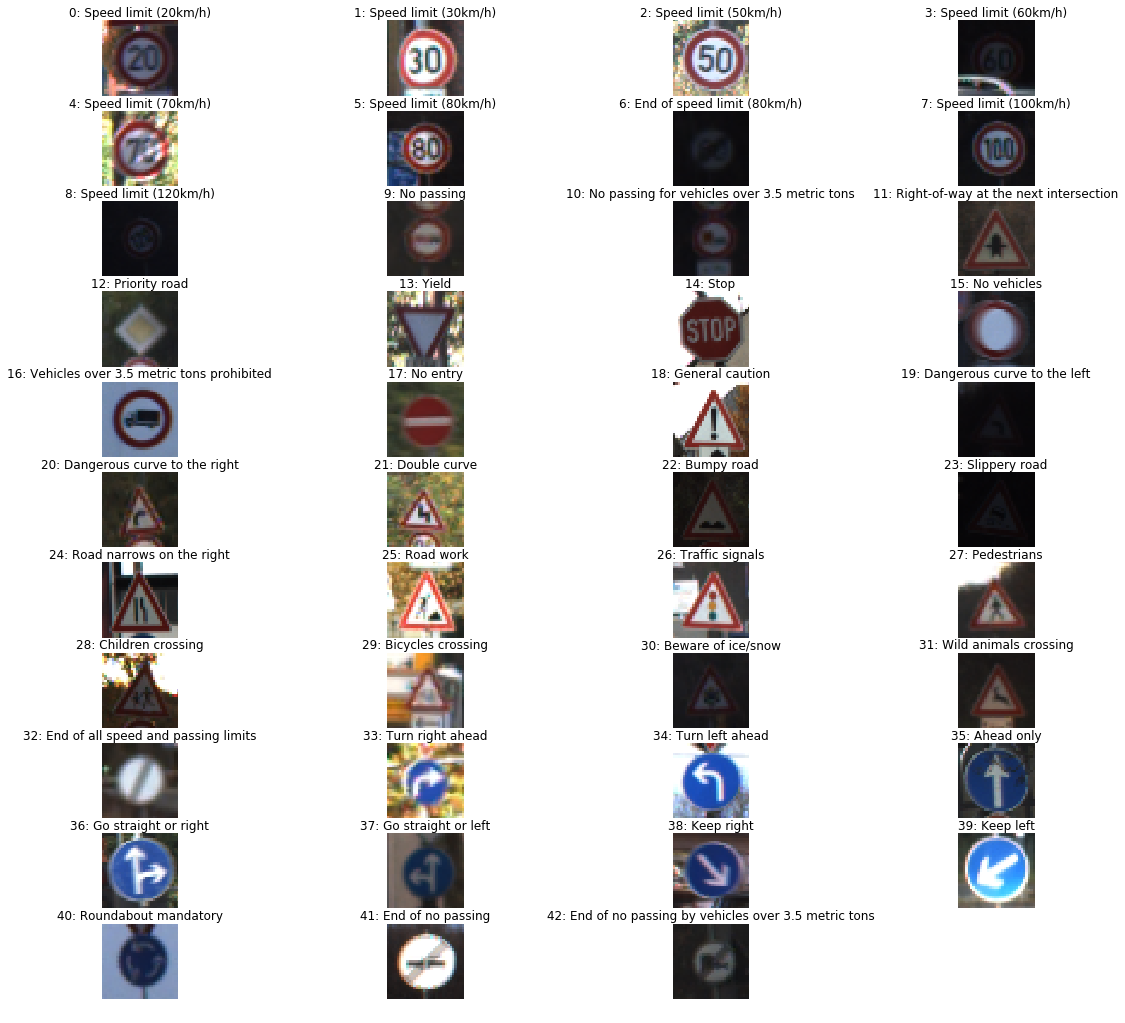
\includegraphics[width=0.8\linewidth]{images_and_labels}
	\caption{Images and Labels}
	\label{fig:images_and_labels}
\end{figure}



\section{Design and Test a Model Architecture}%
\label{sec:design_and_test_a_model_architecture}

\textbf{Describe how you preprocessed the image data. What techniques were chosen and why did you choose these techniques?}


At the beginning I used the Function~\ref{lst:old_pre_process_function} to pre-process the data:


\begin{listing}
\begin{minted}[linenos,numbersep=5pt,frame=lines,framesep=2mm]{python}
IMAGE_SIZE = 32

def tf_resize_images(images):
    X_data = []
    tf.reset_default_graph()
    X = tf.placeholder(tf.float32, (None, None, 3))
    tf_img = tf.image.per_image_standardization(X)
    tf_img = tf.image.rgb_to_grayscale(tf_img)
    with tf.Session() as sess:
        sess.run(tf.global_variables_initializer())
        for image in images:
            output_image = sess.run(tf_img, feed_dict = {X: image})
            X_data.append(output_image)

    X_data = np.array(X_data, dtype = np.float32) # Convert to numpy
    return X_data


## And the implementation would be

X_train = tf_resize_images(X_train)

\end{minted}
\caption{Old Pre-process function}
\label{lst:old_pre_process_function}
\end{listing}

But, I don't know why it constantly gave me an \texttt{TypeError: Cannot interpret feed\_dict as Tensor: The name 'save/Const:0' refers to a Tensor which does not exist ...}.

That's the reason why I end up using plain \texttt{numpy} to sum up the channels to convert to greyscale and normalize the images. I think there is some problem with the sessions or the variables when using Tensorflow for pre-processing. If you can tell why that could be helpful in the future.


\textit{After review: The reason why I used the greyscale step is because the only thing that matters in the sign are the shapes. In fact, there's a lot of similarity between the colors of the signs so it was better to just work with the shapes. I normalized the data to get approximately zero mean and equal variance. Another thing is that this is better so the optimization process could converge faster.}



\textbf{2. Describe what your final model architecture looks like include model type, layers, layer sizes, etc.}




\begin{table}[htpb!]
	\centering
	\caption{Model Architecture}
	\label{tab:model_arc}
	\begin{tabular}{|c|c|}
	\hline
	 Layer		& Description \\
	 \hline
	 \hline
	 Input		& 32x32x1 Greyscale img \\
	 \hline
	 Conv 5x5	& 1x1 stride, VALID padding, outputs 28x28x12 \\ 	
	 \hline
	 Relu		& \\
	 \hline
	 Max pool	& 2x2 strides, outputs 14x14x12 \\
	 \hline
	 Conv 5x5	& 1x1 stride, VALID padding, outputs 10x10x32 \\
	 \hline
	 Relu		& \\
	 \hline
	 Max pool & 2x2 strides, outputs 5x5x32 \\
	 \hline
	 Flatten	& \\
	 \hline
	 Dropout	& keep\_prob = 0.5 when training. \\
	 \hline
	 Fully Connected & Input: 800. Output: 256 \\
	 \hline
	 RELU		& \\
	 \hline
	 Dropout	& keep\_prob = 0.5 when training. \\
	 \hline
	 Fully Connected & Input. 256. Output: 128 \\
	 \hline
	 RELU & \\
	 \hline
	 Dropout	& keep\_prob = 0.5 when training. \\
	 \hline
	 Fully Connected & Input: 128. Output: 43 \\
	 \hline
	 \hline

	\end{tabular}
\end{table}


\textbf{3. Describe how you trained your model.}

The learning rate I used was 0.0005, the number of epochs was 30 and the \texttt{batch\_size = 128}. 


For the loss I used the function \texttt{tf.nn.softmax\_cross\_entropy\_with\_logits\_v2} with the one hot encoded values as labels.\footnote{In particular, I believe it would be interesting to address using the embeddings approach mentioned in the lectures.}



\textbf{4. Describe the approach taken for finding a solution and getting the validation set accuracy to be at least 0.93.}


My validation accuracy was 0.969 and the Test accuracy was 0.958. 

After review: the Process was:


	\begin{itemize}
		\item I search through different kernel sizes and depth.
		\item I try higher depth of the kernels to see if they can extract more information in the images but that was not the case. 
		\item After trying different combinations without success (the accuracy on the validation set was below 70 \% and it looked like there's won't be much improvement besides how much I increase the number of epochs) I ended up with the same architecture as LeNet.
		\item Another thing I tried, was to add more fully connected layers at the end but that was useless too.
		\item After I decided to stick with the LeNet architecture, I added dropout to every fully connected layer to avoid overfitting, that gave me more accuracy in the validation set confirming that I was overfitting in the train set. 
		\item In the optimization process: At the beginning I used a very higher learning rate so I ended up with the problem mentioned in the lectures of faster convergence but to a lower loss. So I decreased the learning rate.
	\end{itemize}







With the architecture, I was interested in playing with the size of the Convolutional kernels, strides, etc. At the end, it seems obvious to me that I don't have an idea of the particular things that make a particular architecture to work. This is something I will dive into in the future. 




\section{Test a Model on New Images}%
\label{sec:test_a_model_on_new_images}

\subsubsection{Choose five German traffic signs from the web}%
\label{ssub:choose_five_german_traffic_signs_from_the_web}

Here are the images from the web used after pre-processing:
\begin{figure}[htpb]
	\centering
	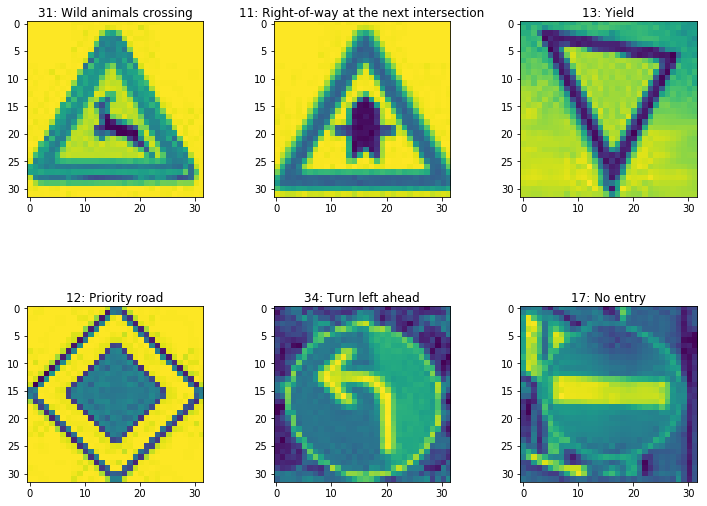
\includegraphics[width=0.8\linewidth]{web_images}
	\caption{Web Images}
	\label{fig:web_images}
\end{figure}


\textit{Review: }The test accuracy on the images was 1.00. This is mainly because this are pretty basic images. They are well centered and they have no noise on them. This made easy to my model classify the images.  








In the Figure~\ref{fig:top_k} we can see the top 5 Softmax Probabilities for each images with the values. This tells us that the confidence of the model is pretty high. The first column is the image with the highest probability, the second is the 2nd guess and so on. Each input image is in each row. 


This is a pretty useful tool to check the similarities between the images with the highest probability.


\begin{figure}[htpb!]
	\centering
	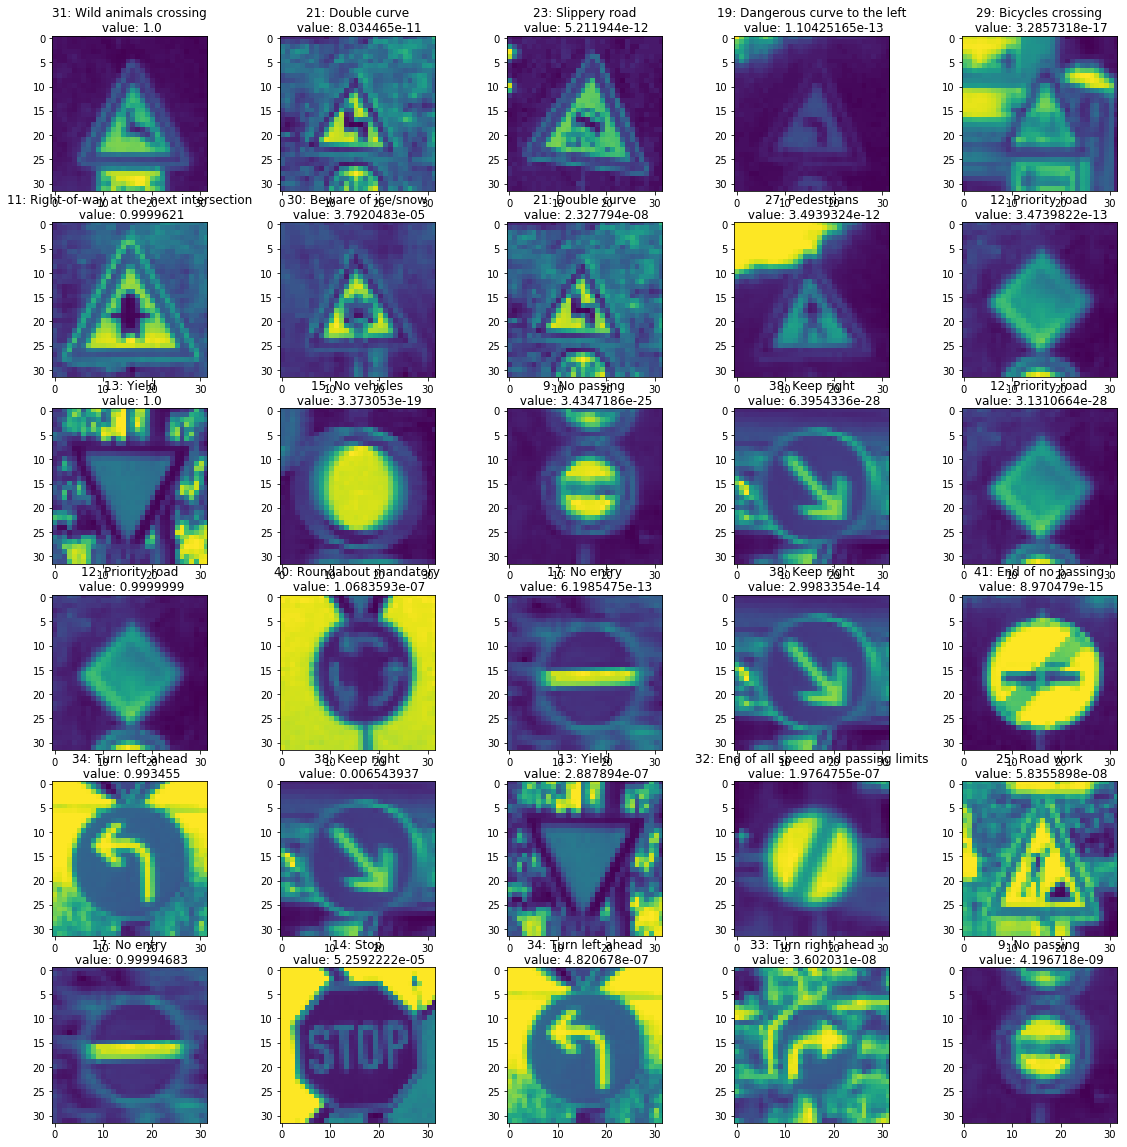
\includegraphics[width=0.8\linewidth]{top_k}
	\caption{Top K}
	\label{fig:top_k}
\end{figure}






The output from the activations are in the Figure~\ref{fig:feature_map}. 


\begin{figure}[htpb!]
	\centering
	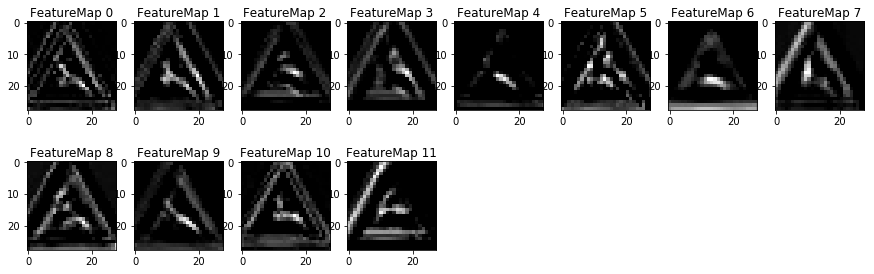
\includegraphics[width=0.8\linewidth]{feature_map}
	\caption{Feature Map}
	\label{fig:feature_map}
\end{figure}




\section{Discussion}%
\label{sec:discussion}


The things I would like to try in the future or some areas where I thing I can improve the implementation of this model are:


\begin{itemize}
	\item Augment the data. 
	\item Use tensorboard.
	\item \textbf{Try to understand better why some particular architectures work}
	\item Use the embeddings approach instead of one hot encoded labels. 
\end{itemize}




\end{document}
